\documentclass{article} 

\usepackage{graphicx}
\usepackage{amsmath}
\usepackage{units}

\begin{document}

\section{Elecci\'on de $f_p$}

Para determinar $f_p$, se busc\'o minimizar este valor a fin de filtrar la mayor cantidad de ruido posible, pero teniendo en cuenta tambi\'en la necesidad de recuperar las se\~nales originales. Se estudió, pues, el espectro de las señales que se utilizarían en la entrada, a saber: un seno en $f_0=$500Hz, un $\nicefrac{3}{2}$ seno en la misma frecuencia, y una exponencial decreciente de per\'iodo 10s, as\'i como una se\~nal de AM. \par 

La primera de estas se\~nales, el seno, nos permite determinar que el filtro antialiasing debe dejar pasar al menos se\~nales de 500Hz. Por otro lado, la se\~nal de AM es:
\[ x(t) = \frac{1}{2} \cdot \cos{\left(2\pi\cdot 1.8f_0 \cdot t\right)} + \cos{\left(2\pi\cdot 2f_0 \cdot t\right)} +\frac{1}{2} \cdot \cos{\left(2\pi\cdot 2.2f_0 \cdot t\right)} \]

De esto sabemos que $f_p$ debe ser al menos $2.2f_0=1.1$kHz. Para dejar un margen de error, consideramos por ahora que $f_p$ debe ser al menos 1.5kHz.

En cuanto a la se\~nal exponencial:
\[ x(t) = e^{-|t|}, \quad -5 \leq t \leq 5 \]

La frecuencia fundamental de la misma es 0.1Hz, con lo cual teniendo en cuenta la restricci\'on anterior, sabemos que van a pasar m\'as de 5000 de sus arm\'onicos, con lo cual en principio esta se\~nal no ser\'ia un problema. Para comprobar esta suposici\'on, se obtuvieron los coeficientes de la serie exponencial de Fourier de esta funci\'on, resultando:
\[ X_n = \frac{2}{T} \cdot \frac{1 - (-1)^n \cdot e^{-\nicefrac{T}{2}}}{1 + \left(\frac{2\pi n}{T}\right)^2} \]

Sabiendo que la potencia correspondiente al en\'esimo arm\'onico es $2 \cdot |X_n|^2$ (salvo para $n=0$, donde no se duplica el valor del coeficiente), se confirm\'o que la misma se hace absolutamente despreciable a partir del octavo arm\'onico, hasta donde se encuentra m\'as del 99\% de la potencia. Por lo tanto, esta se\~nal no impone restricciones al filtro antialiasing.

\begin{figure}[htb]     
	\centering     
	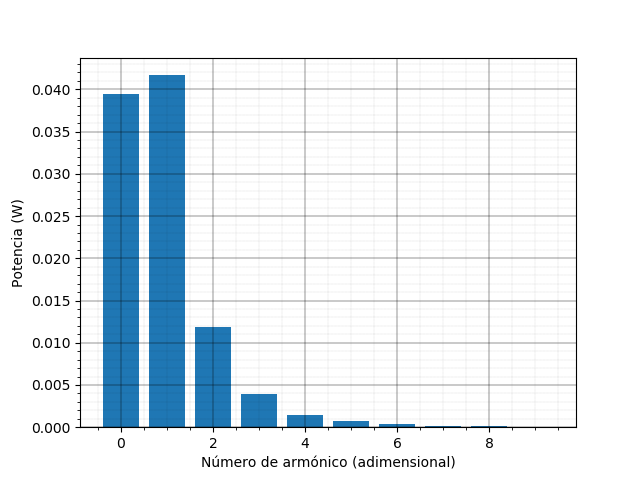
\includegraphics[scale=0.45]{armonicos/exp_potencia.png}     
	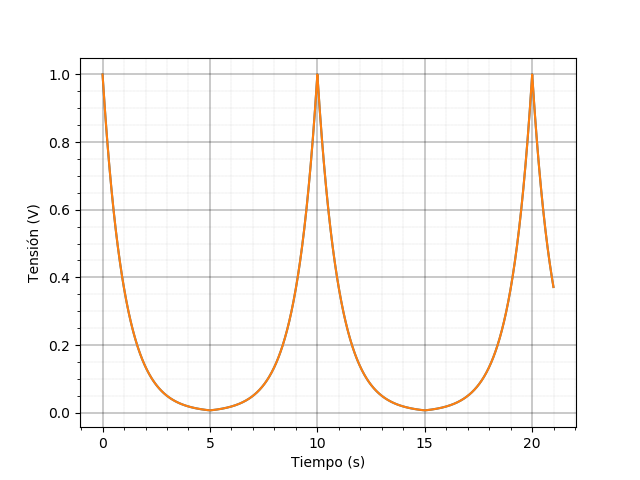
\includegraphics[scale=0.45]{armonicos/exp_funcion.png}     
	\caption{Potencia en funci\'on del n\'umero de arm\'onico de la se\~nal exponencial (izquierda), y se\~nal reconstruida con 50 arm\'onicos (derecha), superpuesta a la se\~nal original (no llegan a distinguirse).}     
	\label{fig:armonicos_exp} 
\end{figure}

Considerando que incluso con una frecuencia 100 veces mayor, de 10Hz, se recuperan 50 arm\'onicos y la se\~nal se recupera de manera virtualmente completa (como se observa en la figura \ref{fig:armonicos_exp}), se decidi\'o trabajar esta frecuencia m\'as r\'apida, a fin de no tener que esperar 10 segundos para medir un per\'iodo.

En el caso del $\nicefrac{3}{2}$ seno, la frecuencia fundamental es en cambio 500Hz, con lo cual por un filtro con $f_p=1500\mathrm{Hz}$ pasar\'ia la fundamental y los siguientes 2 arm\'onicos. Para analizar el espectro en este caso se utiliz\'o la serie trigonom\'etrica de Fourier, obteni\'endose:
\[ a_0 = \frac{2}{3\pi},\quad a_n=\frac{12}{\pi} \cdot \left(\frac{1}{9-4n^2}\right) , \quad b_n=0 \]

\begin{figure}[htb]     
	\centering     
	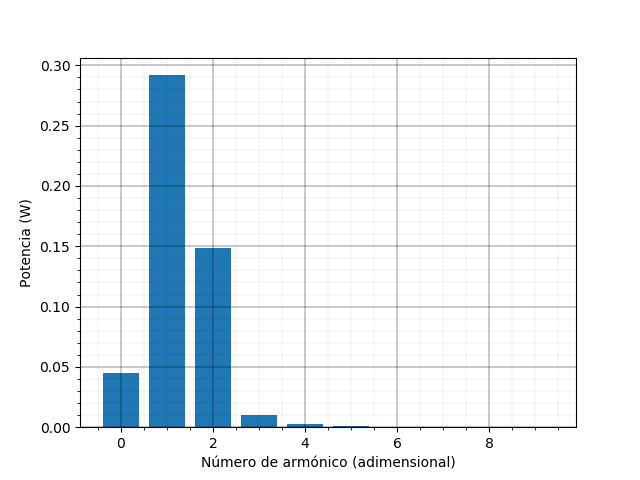
\includegraphics[scale=0.45]{armonicos/32seno_potencia.png}     
	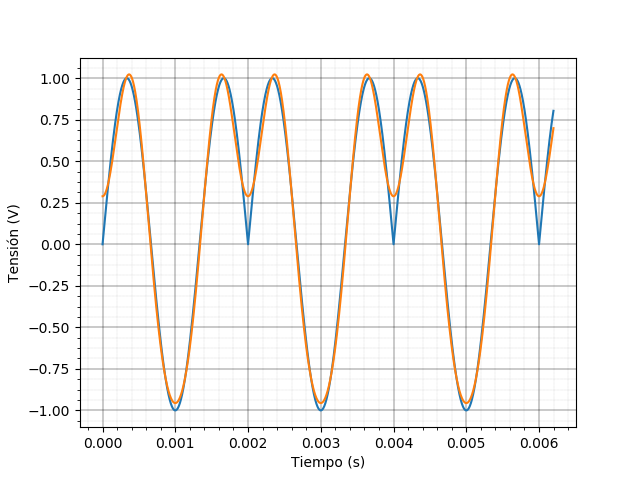
\includegraphics[scale=0.45]{armonicos/32seno_funcion.png}     
	\caption{Potencia en funci\'on del n\'umero de arm\'onico del \nicefrac{3}{2} (izquierda), y se\~nal reconstruida con 3 arm\'onicos incluyendo la fundamental (derecha, naranja), supuerpuesta a la se\~nal original (azul).}     
	\label{fig:armonicos_32} 
\end{figure}

Se obtuvo, pues, que hasta 500Hz se tiene el 67\% de la potencia, hasta 1kHz el 97\%, y hasta 1.5kHz el 99\%. Por lo tanto, siendo que con $f_p=1.5\mathrm{kHz}$ se puede conservar m\'as del 99\% de la potencia de las 3 se\~nales de entrada, se utiliz\'o este valor, con el cual se recupera la se\~nal tal como se observa en la figura \ref{fig:armonicos_32}.

\end{document} 